%this is chapter about the introduction about the problem in my thesis: it is the cadinality estimation to query performance.

\chapter{QUERY OPTIMIZATION.}\label{chapter:query optimization}
\section{HOW IS A QUERY EXECUTED?}
\subsection{The main steps to execute a query.}
{
\begin{flushleft}
{\justify
There are five main components in Postgresql architecture \cite{PostgreSQL internals}:
\begin{itemize}
\item The parser -  parse the query string
\item The rewriter - apply rewrite rules
\item The optimizer - determine an efficient query plan
\item The executor - execute a query plan
\item The utility processor - process DDL like \bfseries CREATE TABLE
\end{itemize}
\par }
{\justify
Firgure 2.1 shows the architecture diagram of query executor in Postgresql. In the first step, query string is parsed to parse tree in the parser. After that, parse tree is analyzed its semantic and transformed to Query node. In the next step PostgreSQL processes DDL (Data Definition Language) like {\bfseries CREATE TABLE} or apply rewrite rules in rewriter. Before going to executor, query tree is used to produce a query plan.
\par }
\begin{figure}[H]
\centering
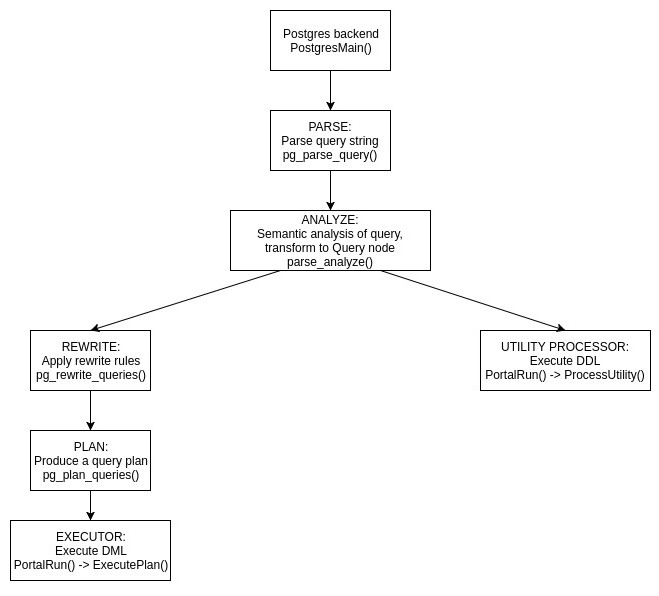
\includegraphics[width=1.0\textwidth]{architecture_diagram.jpg}
\caption{Architecture diagram of Postgresql.}
\end{figure}
\end{flushleft}
}
\subsection{Parser}
\begin{flushleft}
{\justify
The parser \cite{Flow of a select statement} has to check the query string (which arrives as plain ASCII text) for valid syntax. If the syntax is correct a parse tree is built up and handed back; otherwise an error is returned. It is defined in gram.y and scan.l which are built by using the Unix tools yacc and lex.
\par}
\vspace{0.5cm}
{\justify
It turns out that PostgreSQL uses the same parsing technology that Ruby does, a parser generator called {\bfseries Bison}. Bison runs during the PostgreSQL C build process and generates parser code based on a series of grammar rules. The generated parser code is what runs inside of PostgreSQL when we send it SQL commands. Each grammar rule is triggered when the generated parser finds a corresponding pattern or syntax in the SQL string, and inserts a new C memory structure into the parse tree data structure.
\par }
\vspace{0.5cm}
{\justify
Figure 2.2 is an example about the parse tree of the query: \\
\newpage\begin{verbatim}
SELECT * FROM movies 
WHERE country = 'France' ORDER BY id ASC LIMIT 1
\end{verbatim}
%\item\bfseries 

\begin{figure}[H]
\centering
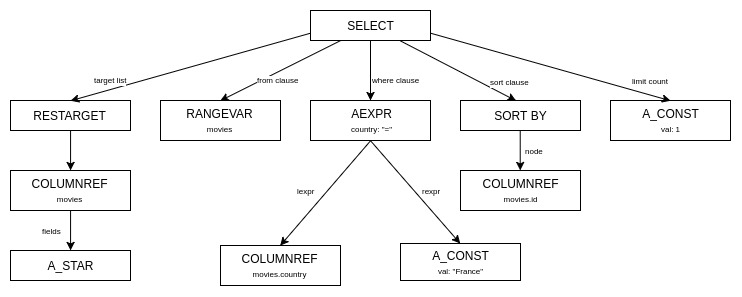
\includegraphics[width=1.0\textwidth]{parser_example.jpg}
\caption{An example about parse tree.}
\end{figure}
}
\end{flushleft}
\subsection{Rewriter}
\begin{flushleft}
\justify
Once PostgreSQL has generated a parse tree, it then converts it into another tree using a different set of nodes. This is known as the query tree. The parts of a query tree \cite{PostgreSQL internals} are:
\begin{itemize}
\item The command type: This is a simple value telling which command (SELECT, INSERT, UPDATE, DELETE) produced the query tree.
\item The range table: The range table is a list of relations that are used in the query. In a SELECT statement these are the relations given after the FROM key word.
\item The result relation: This is an index into the range table that identifies the relation where the results of the query go.
\item The target list: The target list is a list of expressions that define the result of the query. In the case of a SELECT, these expressions are the ones that build the final output of the query. They correspond to the expressions between the key words SELECT and FROM (* is just an abbreviation for all the column names of a relation. It is expanded by the parser into the individual columns, so the rule system never sees it.).
\item The qualification: The query's qualification is an expression much like one of those contained in the target list entries. The result value of this expression is a Boolean that tells whether the operation (INSERT, UPDATE, DELETE, or SELECT) for the final result row should be executed or not. It corresponds to the WHERE clause of an SQL statement.
\item The join tree: The query's join tree shows the structure of the FROM clause. For a simple query like SELECT ... FROM a, b, c, the join tree is just a list of the FROM items, because we are allowed to join them in any order. But when JOIN expressions, particularly outer joins, are used, we have to join in the order shown by the joins. In that case, the join tree shows the structure of the JOIN expressions. The restrictions associated with particular JOIN clauses (from ON or USING expressions) are stored as qualification expressions attached to those join-tree nodes. It turns out to be convenient to store the top-level WHERE expression as a qualification attached to the top-level join-tree item, too. So really the join tree represents both the FROM and WHERE clauses of a SELECT.
\item The others: The other parts of the query tree like the ORDER BY clause
\end{itemize}
{\justify
Figure 2.3 is an example about the query tree of the query:
\begin{verbatim}
SELECT * FROM movies 
WHERE country = 'France' ORDER BY id ASC LIMIT 1
\end{verbatim}
}
\begin{figure}[H]
\centering
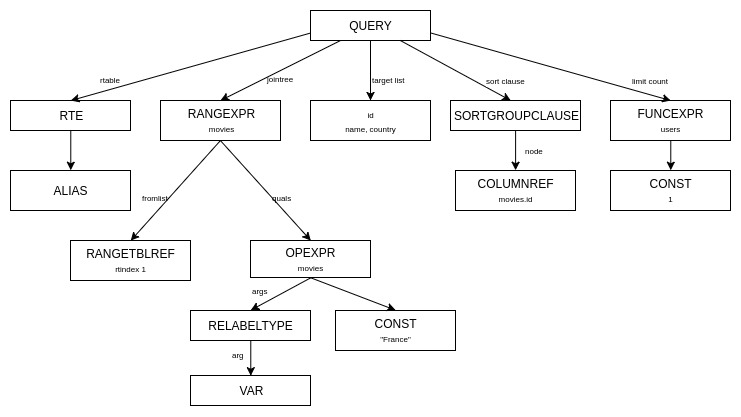
\includegraphics[width=1.0\textwidth]{example_querytree.jpg}
\caption{An example about query tree.}
\end{figure}
\end{flushleft}
\subsection{Planner}
\begin{flushleft}
{\justify
The task of the planner \cite{Flow of a select statement} is to create an optimal execution plan. A query tree of a SQL plan can be actually executed in a wide variety of different ways, each of them will produce the same of results. If it is computationally feasible, the query optimizer will examine each of these possible execution plans, ultimately selecting the execution plan that is expected to run the fastest.
\par }
\vspace{0.5cm}
{\justify
The planner's search procedure actually works with data structures called paths, which are simply cut-down representations of plans containing only as much information as the the planner needs to make its decisions. After the cheapest path is determined, a full-fledged plan tree is built to pass to the executor. This represents the desired execution plan in sufficient detail for the executor to run it.
\par }
{\justify
Firgure 2.4 is the full-fledged plan tree of the query:
\begin{verbatim}
SELECT * FROM movies 
WHERE country = 'France' ORDER BY id ASC LIMIT 1
\end{verbatim}
\par }
\begin{figure}[H]
\centering
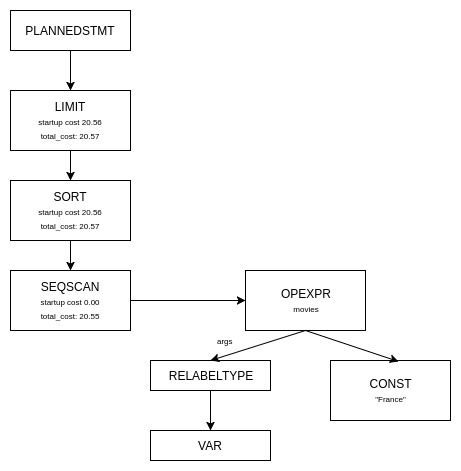
\includegraphics[width=1.0\textwidth]{plan_tree_example.jpg}
\caption{An example about full-fledged plan tree.}
\end{figure}
\vspace{0.5cm}
\end{flushleft}
\subsection{Executor}
{\justify
The executor \cite{PostgreSQL internals} takes the plan handed back by the planner and recursively processes it to extract the required set of rows. This is essentially a demand-pull pipeline mechanism. Each time a plan node is called, it must deliver one more row, or report that it is done delivering rows.
\par }
\vspace{0.5cm}
{\justify
To provide an example, assume that the top node is a MergeJoin node. Before any merge can be done two rows have to be fetched (one from each subplan). So the executor recursively calls itself to process the subplans (it starts with the subplan attached to lefttree). The new top node (the top node of the left subplan) is, let's say, a Sort node and again recursion is needed to obtain an input row. The child node of the Sort might be a SeqScan node, representing actual reading of a table. Execution of this node causes the executor to fetch a row from the table and return it up to the calling node. The Sort node will repeatedly call its child to obtain all the rows to be sorted. When the input is exhausted (as indicated by the child node returning a NULL instead of a row), the Sort code performs the sort, and finally is able to return its first output row, namely the first one in sorted order. It keeps the remaining rows stored so that it can deliver them in sorted order in response to later demands.
\par}
\vspace{0.5cm}
{\justify
The MergeJoin node similarly demands the first row from its right subplan. Then it compares the two rows to see if they can be joined; if so, it returns a join row to its caller. On the next call, or immediately if it cannot join the current pair of inputs, it advances to the next row of one table or the other (depending on how the comparison came out), and again checks for a match. Eventually, one subplan or the other is exhausted, and the MergeJoin node returns NULL to indicate that no more join rows can be formed.
\par }
\vspace{0.5cm}
{\justify
Complex queries can involve many levels of plan nodes, but the general approach is the same: each node computes and returns its next output row each time it is called. Each node is also responsible for applying any selection or projection expressions that were assigned to it by the planner.
\par }
\vspace{0.5cm}
\section{QUERY OPTIMIZATION.}
\subsection{Introduction.}
{\justify
{\bfseries Query optimization} is a function of relational database management systems. The query optimizer attempts to determine the most efficient way to execute a given query by considering the possible query plans. Therefore, it is belong to planner stage.
\par }
\vspace{0.5cm}
{\justify
There is a trade-off between the amount of time spent figuring out the best query plan and  the quality of the choice; the optimizer may not choose the best answer on its own. Different qualities of database management systems have different ways of balancing these two. Cost-based query optimiers, such as PostgreSQL optimizer, evaluate the resource footprint of various query plans and use this as the basis for plan selection. They assign an estimated "cost" to each possible query plan, and choose the plan with the smallest cost.  Costs are used to estimate the runtime cost of evaluating the query, in terms of the number of I/O operations required, CPU path length, amount of disk buffer space, disk storage service time, and interconnect usage between units of parallelism. The set of query plans examined is formed by examining the possible access paths (e.g., primary index access, secondary index access, full file scan) and various relational table join techniques (e.g., merge join, hash join). The search space can become quite large depending on the complexity of the SQL query. There are two types of optimization. These consist of logical optimization which generates a sequence of relational algebra to solve the query and physical optimization which is used to determine the means of carrying out each operation.
\par }
\vspace{0.5cm}
\subsection{The query optimizer of PostgreSQL}
{\justify As i mentioned above, PostgreSQL's optimizer is a cost-based optimizer, so it chooses the plan that have the lowest estimated processing cost to execute. PostgreSQL's optimizer determines the cost of executing a query plan based on two main factors: 
\begin{itemize}
\item Cardinality estimation: the total number of rows processed at each level of a query plan, referred to as the cardinality of the plan.
\item Cost model: the cost model of the algorithm dictated by the operators used in the query
\end{itemize}
The first factor, cardinality, is used as an input parameter of the second factor, the cost model. Therefore, improving cardinality estimation leads to better estimated costs and, in turn, faster execution plans.
\par }
\subsection{PostgreSQL's cardinality estimator and its limitations.}
\subsubsection{PostgreSQL's cardinality estimator}
{\justify
Postgresql's optimizer follows the traditional textbook architecture. The cardinalities of base tables are estimated using histograms (quantile statistics), most common values with their frequencies, and domain cardinalities (distinct value counts). These per-attribute statistics are computed by the analyze command using a sample of the relation. For complex predicates, histograms can not be applied. To combine conjunctive predicates for the same table, PostgreSQL simply assumes independence and multiplies the selectivities of the individual selectivity estimates 
\par }
\vspace{0.5cm}
{\justify
The assumptions that PostgreSQL's cardinality estimator based on:
\begin{itemize}
\item Independence: predicates on attributes (in the same table or from joined tables) are independent.
\item Uniformity: all values, except for the most-frequent ones, are assumed to have the same number of tuples
\item Priciple of inclusion: the domains of the join keys overlap such that the keys from the smaller domain have matches in the larger domain.
\end{itemize}
The formula \cite{JOB} that is used to estimate result sizes of joins show these assumptions:\\
{\justify
\centering $\vert T_{1} \bowtie_{x=y} T_{2}\vert$ = $\frac{{\vert {T_{1}\vert}}{\vert {T_{2}\vert}}}{max(dom(x),dom(y))}$ 
\par }
\vspace{0.5cm}
Where $T_{1}$ and $T_{2}$ are arbitrary expresions and dom(x) is the domain cardinality of attribute x, i.e., the number of distinct values of x.
\par }
\vspace{0.5cm}
\subsubsection{The limitation of PostgreSQL's cardinality estimator}
{\justify
\begin{itemize}
\item Correlated data : Correlated data \cite{CE limitations} between relations can lead to the bad cardinality estimation of PostgreSQL executor. To be more specific, i use the example below to demonstrate the impact of the correlation between relations to cardinality estimation of PostgreSQL:
\begin{verbatim}
SELECT * FROM Products where Company = 'Toyota' and Brand = 'Civic'
\end{verbatim}
When you look at this query, you will know immediately how many rows are returned. The number of returned results is zero because the company Toyota doesn't have Civic brand car. But as i metioned above, the PostgreSQL's optimizer uses the assumptions (uniformity, independence, inclusion, ad hoc constants), so it looks at each search predicate indepedently. \par 
In the first step the cardinality estimation is done for the predicate {\bfseries Company = 'Toyota'}. After that, the optimizer produces a cardinality estimation for other predicate {\bfseries Brand = 'Civic'}. And finally both estimations are multiplied by each other to produce the final estimation. When the first predicate produces a cardinality selectivity of 0.4 and the second one produces a cardinality selectivity of 0.4, the final cardinality selectivity will be 0.16 (0.4*0.4) instead of 0.0 as the fact. The PostgreSQL's optimizer handles every predicate on its own without any correlation between relations.
\end{itemize}
}